\documentclass[noindent]{scrartcl}

\usepackage{../Header/header}

\begin{document}


%----------------------------------------------------------------------------------------
%	NAME AND CONTACT INFORMATION SECTION
%----------------------------------------------------------------------------------------

\thispagestyle{empty}
\begin{tikzpicture}[remember picture,overlay]
    \node[align=center] at ([yshift=-7cm]current page.north)%
         {\huge \spacedallcaps{Curriculum Vitae}};
    % cover photo
    \node[align=center] (image) at ([yshift=-13cm]current page.north) %
         {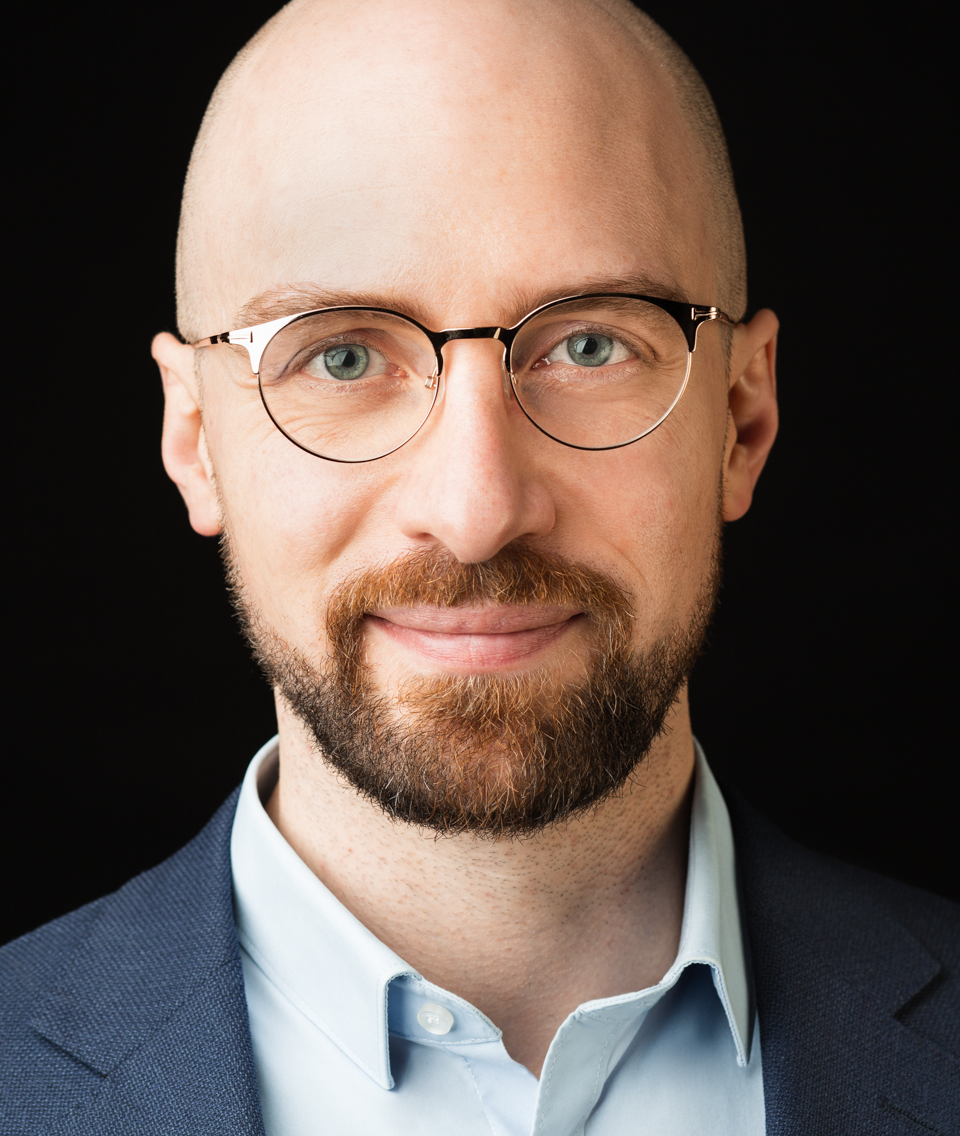
\includegraphics[width=75mm,height=105mm]{Foto}};
    % name and address
    \node[align=center] (name) at ([yshift=-19cm]current page.north) %
         {\Huge \textcolor{blaze}{\spacedallcaps{Julian Müller}}};
    \node[align=center] at ([yshift=-20.2cm]current page.north) %
         {\textcolor{blaze}{\spacedallcaps{Maschinenbau, (B.E.)}}};
    \node[align=center] at ([yshift=-21.2cm]current page.north) %
         {\textcolor{blaze}{\spacedallcaps{Logik, (M.A.)}}};
    \node[align=left] at ([xshift=0.3cm,yshift=-25cm]current page.north) % 
         {\color{textgray}
			\begin{tabular}{lr}
             Geburtsdatum & 29 Oktober 1984 \vspace{0.5em} \\

             Geburtsort & 77694 Kehl \vspace{0.5em} \\

             Email & \href{mailto:jul.mue@hotmail.de}{jul.mue@hotmail.de} \vspace{0.5em} \\

             Website & \href{https://julmue.github.io}{julmue.github.io} \vspace{0.5em} \\

             Telefon & +49 176 55509278 \vspace{0.5em}  \\

             Adresse & Josef-Gottwald-Stra\ss e 1 \vspace{0.5em}  \\
                       & 77654 Offenburg \\
            \end{tabular}
         };
\end{tikzpicture}
%\thispagestyle{empty} % Stop the page count at the bottom of the first page

% Your name
\newpage
%\begin{cv}{\spacedallcaps{Julian Müller}}\vspace{1.5em} 

%----------------------------------------------------------------------------------------
%	EDUCATION
%----------------------------------------------------------------------------------------

\begin{cv}

\topic{Ausbildung}

\NewEntry{2013-2016}{Logik (M.A.)}{Universität Leipzig}

\Description{\MarginText{\href{http://www.sozphil.uni-leipzig.de/cm/logik/}{Master Logik}\\
(Endnote: 1.6)}%
%Abschluss: 1.6 (angestrebt)\newline%
Spezialisierungen:
\EvenThree
    {\isym\ \textit{Constraint-Programmierung}}%
    {\isym\ \textit{Parakonsistente Logiken}}%
    {\isym\ \textit{Wissensrepräsentation}}
{Abschlussarbeit (Note 1.0): \textit{Das untypisierte Lambdakalkül und seine Anwendung}\newline
\isym\ \textit{In der Informatik}: Als Grundlage funktionaler Programmiersprachen\newline
\isym\ \textit{In der Beweistheorie}: Curry-Howard-Lambek-Isomorphismus\newline
\isym\ \textit{In der Mathematik}: Als interne Sprache kartesisch geschlossener Kategorien\newline
Betreuer: Dr.~Peter \textsc{Steinacker}, Prof.~Thomas \textsc{Bartelborth}}\newline
Abgabe: 14.07.2016}

%------------------------------------------------

\NewEntry{2008-2013}{Maschinenbau (B.E.)}{RFH Köln}

\Description{\MarginText{Bachelor Maschinenbau\\(Endnote: 1.8)}%
Spezialisierungen:
\EvenThree%
    {\isym\ \textit{Technische Optik / Lasertechnik}}%
    {\isym\ \textit{Mechatronik}}%
    {\isym\ \textit{Programmieren in C}}%
Abschlussarbeit (Note 1.0): \textit{Verschlei\ss erkennung bei Werkzeugen im Tunnelbau}\newline
\isym\ \textit{Entwicklung, Bau und Inbetriebnahme eines Laserscanners zur Verschlei\ss messung}\newline
\isym\ \textit{Vergleich von Verfahren der industriellen Bildverarbeitung (2d/3d)}\newline
\isym\ \textit{Projektspezifische Analyse geometrischer und logistischer Randbedingungen von\\ 
               \hspace{0.8em}Vortriebsprozessen im maschinellen Tunnelbau}\newline
Betreuer: Prof.~Werner \textsc{Simon}, Prof.~Marcus \textsc{Scholl}}

\NewEntry{2004-2007}{Event Organizer}{Angell Institut Freiburg}

\Description{\MarginText{Event Organizer}%
Ausbildung zum \textit{International Event Organizer}.}

%----------------------------------------------------------------------------------------
%	WORK EXPERIENCE
%----------------------------------------------------------------------------------------

\topic{Berufspraxis}

% ------------------------------------------------------------------------------
% ------------------------------------------------------------------------------
% ------------------------------------------------------------------------------
\NewEntry{04/2012-07/2012}{Werkstudent (F\&E)}{Herrenknecht AG}

\Description{\MarginText{Werkstudent\\Forschung \& Entwicklung}%
Abschluss des Forschungsprojekts aus der Bachelorarbeit:\newline
Planung, Konstruktion und Inbetriebnahme eines Versuchsstandes zur Lasertriangulation:\newline
\isym\ Berechnung der optischen Komponenten und der Antriebseinheit\newline
\isym\ Planung, Realisierung und Inbetriebnahme des Prototypen
}

\NewEntry{10/2010-04/2012}{Bachelorand (F\&E)}{Herrenknecht AG}

\Description{\MarginText{Bachelorand\\Forschung \& Entwicklung}%
Projektbezogene Untersuchung von Verfahren der optischen Messtechnik:\newline
\isym\ Test und Untersuchung von Verfahren zur Tiefenbildgewinnung\newline
\isym\ Untersuchung von Verfahren zur Merkmalsextraktion in Grauwertbildern\newline
\isym\ Analyse von Prozessen im Vortriebszyklus beim Tunnelbau\newline
\isym\ Anforderungsermittlung und Konzeption eines Messsystems
}

\NewEntry{09/2010-03/2011}{Praktikant (F\&E)}{Herrenknecht AG}
     
\Description{\MarginText{Praktikant\\Forschung \& Entwicklung}%
Entwicklung von Konzepten zum maschinellen Tunnelvortrieb:\newline
\isym\ Projekt: maschineller Tunnelvortrieb in der nuklearen Forschung\newline
\isym\ Maschinenkonzept: Aufweitung bestehender Tunnel unter \\
       \hspace{0.85em}Aufrechterhaltung des Stra\ss en- und Bahnverkehrs
}


\NewEntry{01/2009-09/2009}{Tutor (Mathematik)}{RFH Köln}

\Description{\MarginText{Tutor\\Mathematik}%
Tutorium für Ingenieursmathematik:\newline
\isym\ Grundlagen der Ingenieursmathematik\newline
\isym\ Differenzial-/Integralrechnung\newline
\isym\ Vektorrechnung
}

\NewEntry{04/2006-07/2006}{Praktikant (Verwaltung)}{LLombart Export}
     
\Description{\MarginText{Praktikant\\(Spanien)}%
Auslandspraktikum Spanien --- Aufgabenbereich allgemeine Büroarbeiten: 
Administration, Übersetzungen, Ablage
}

% ------------------------------------------------------------------------------
% ------------------------------------------------------------------------------
% ------------------------------------------------------------------------------

\newpage
%----------------------------------------------------------------------------------------
%	Projekte
%----------------------------------------------------------------------------------------
\topic{Software-Projekte}

\NewEntry{Funktionale Programmierung}{Haskell}{\href{https://github.com/julmue/UntypedLambda}{Projektseite}}

\Description{\MarginText{Interpreter}%
Interpreter für das untypisierte Lambdakalkül; 
Die durch das untypisierte Lambdakalkül formalisierte Berechenbarkeit ist äquivalent zur Turing-Berechenbarkeit.
Weiter ist das System Grundlage für funktionale Programmiersprachen und findet Anwendung als 
Zwischensprache (\emph{Intermediate Language}) im Compilerbau.
}

\NewEntry{Funktionale Programmierung}{Haskell}{\href{https://github.com/julmue/lfo}{Projektseite}}

\Description{\MarginText{Interpreter}%
Interpreter für das einfach typisierte Lambdakalkül;
Dieses Kalkül ist das theoretische Fundament statisch typisierte funktionaler
Programmiersprachen und von zentraler Bedeutung in der Beweistheorie.
}

\NewEntry{Constraint Programmierung}{Haskell}{\href{https://github.com/julmue/Clank}{Projektseite}}

\Description{\MarginText{Solver}%
Solver für die parakonsistenten Aussagenlogiken K3, L3, LP, RM sowie für die 
klassische Aussagenlogik.
Diese Logiken werden unter anderem in der Robotik, künstlichen Intelligenz und 
Wissensrepräsentation angewendet.
}

\NewEntry{Constraint Programmierung}{Prolog}{\href{https://github.com/julmue/DpllDimacSatSolver}{Projektseite}}

\Description{\MarginText{SAT-Solver}%
Solver für die klassisch Aussagenlogik (Grundlage: DPLL-Algorithmus);\\
Industrielle Anwendungen findet dieses Verfahren bei der Lösung von
Baubarkeits- und Planungsproblemen sowie im Variantenmanagement.
}

\NewEntry{Beweistheorie}{Haskell}{\href{https://github.com/julmue/HaskellCurryHoward}{Projektseite}}

\Description{\MarginText{Beweistheorie /\\Kombinatoren-bibliothek}%
Der Curry-Howard-Lambek-Isomorphismus ist die zentrale Verbindung von 
funktionaler Programmierung, Logik und Kategorientheorie:
Programme sind konstruktive Beweise, konstruktive Beweise sind Morphismen.
}

%----------------------------------------------------------------------------------------
%	COMPUTER SKILLS
%----------------------------------------------------------------------------------------
\topic{Programmiersprachen}

\Description{\MarginText{Sehr gut} Haskell, Prolog}

\Description{\MarginText{Gut} C, MATLAB, Simulink, OCaml}

\Description{\MarginText{Grundlagen} Scala, SQL, JavaScript/ECMAScript, HTML, CSS, Java, Bash, SMT-Lib}


\topic{Technologien}

\Description{\MarginText{Betriebssysteme} Linux (Ubuntu, Mint, \dots), Windows}

\Description{\MarginText{Versionierung} git}

\Description{\MarginText{Computervision} MathWorks Image Processing Toolbox (MATLAB)}

\Description{\MarginText{Test-Frameworks} XUnit-Frameworks in Java, Haskell, Prolog, C++, C, \dots}


%-------------------------------------------------------------------------------
\topic{Fremdsprachen}

\Description{\MarginText{Sehr gut}Englisch (\emph{verhandlungssicher})}
\Description{\MarginText{Grundlagen}Spanisch}


%-------------------------------------------------------------------------------
\topic{Sonstiges}

\NewEntry{08/2005-03/2006}{Work \& Travel}{Neuseeland}

\Description{\MarginText{Sprachreise\\Englisch}%
Sprach- und Arbeitsreise Neuseeland
}


\end{cv}

\end{document}
